\chapter{Energetic Electron Precipitation and Geospace}

\section{Introduction to Connected Geospace}

The Earth is a complicated place. Natural processes, which occur on vastly different time scales, are all connected to each other and produce the state of the overall system. Only in the last 70 years or so, since the beginning of the space age, has the picture of the Earth as a dynamic system been extended to include the space around it. This space is not empty, and it has structure and dynamics which are very different than processes on Earth, mostly owing to the importance of the electromagnetic force between its constituents. The word used to describe the space around Earth is geospace, so-named because the Earth and its processses are not strictly separated from the space around it. In fact, information, matter, and energy flow between regions which can be separated by great distances, and cause effects which can echo throughout the entire system. In this chapter, I will describe one of the most dramatic ways which this can happen, where energetic particles from space enter the atmosphere and affect it directly. 

Energetic electron precipitation is a process by which electrons depart trapped states in geospace and enter the Earths atmosphere. One of the most brilliant effects that can be caused by this process is able to be seen from the ground on Earth - the northern lights, or Aurora Borealis. There has been a great deal of work done in the last half-century to understand, quantity, and model the processes responsible for creating the Aurroa, but many unanswered questions remain. With the knowledge that the Earth and the space around it are both connected and affect each other, it becomes of great scientific interest to understand the ways which particles and energy move between them. The fact that energetic particle precipitation can have dramatic visual affects on the atmosphere motivates its use as measurable target which can provide a window to the dynamics of the connected system. 

The earth and geospace are not stationary systems. One can draw a loose analogy between their related structure and the anatomy of a living organism. While the system is always in a state of change, there is a consistent structure and organization at the highest levels. In this case, that structure is largely defined by the magnetic field of the Earth, and the magnetic field of the solar wind which interacts with it. Navigation on the surface of the Earth can be accomplished by measuring the direction of the local magnetic field in two dimensions. In geospace, the magnetic field changes significantly over all three dimensions, and, to an extent, in time as well. As charged particles, electrons in geospace are subject to the Lorentz force. This force is always orthogonal to the magnetic field, which is why the magnetic field is such a powerful organizational force in the system. 

The magnetic field of the Earth is due to both internal, and external (space-based) current sources. This field can be conveniently described by the multipole expansion. Figure~\ref{magnetosphere_diagram} shows a model of the magnetic field of the Earth, which takes into account both internal and external sources. Towards the surface, the dipole is a good approximation. Farther away, however, higher-order terms become important and result in a field has a vastly different structure than the dipole description. The magnetic field geometry in Figure~\ref{magnetosphere_diagram} does not imply a steady-state to the system. Rather, this can be thought of as the overall topology of a system which is always in motion. In reality, only some modified version of this picture will be accurate at any particular time. Particularly, at distances which exceed a few Earth radii, the state of the solar wind, through which the Earth is always moving, becomes more important than the current sources internal to the Earth itself. A more accurate picture of the system than Figure~\ref{magnetosphere_diagram} would actually be an animation, with magnetic field lines cascading on the dipole field of the Earth, and reconnecting to form the stretched-out ``tail'' from 10 to hundreds of Earth radii ``downwind''. The description of that process is an entire field of study, and it too, has questions which are currently unanswered.

\begin{figure}[p]
\label{magnetosphere_diagram}
\centering
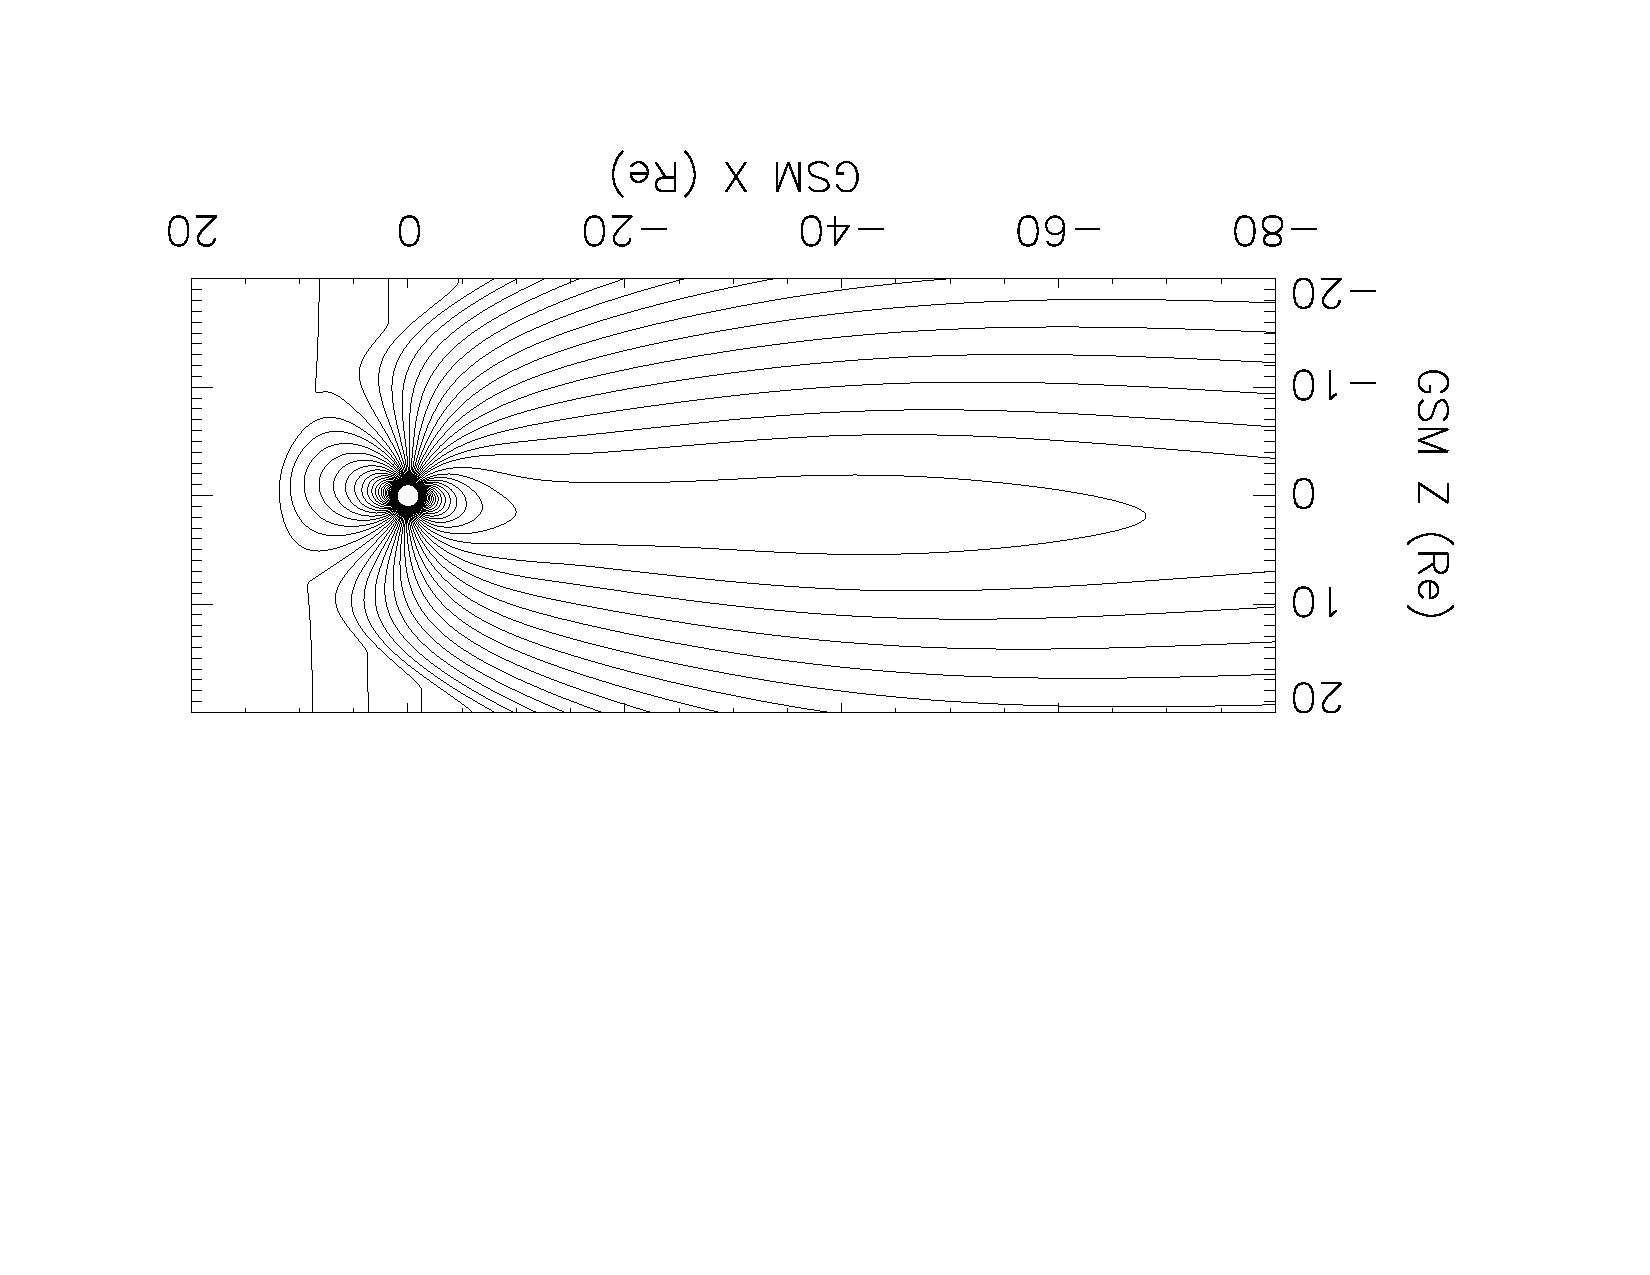
\includegraphics[width=1.1\textwidth,angle=180]{figures/chapter_2/magnetosphere_diagram/magnetosphere_diagram}
\caption{Model of the magnetic field of the Earth which includes effects due to external sources and the solar wind. Coordinates are measured in Earth radii and centered on the Earth. Near to the earth, a dipole field describes the geometry well. Farther away, this changes. }
\end{figure}

Given that electrons in geospace exist, and they are subject to a magnetic field geometry which is complicated and dynamic on the relevant scales, this suggests that the motion of electrons within the system is important to the state of the overall system. This, then, implies that the loss of these particles to the Earths atmosphere, is also important. The goal of this chapter is to describe, in adequate detail, the connection between the precipitation of electrons into the atmosphere and the state of the larger geophysical system. The goal is to advance electron precipitation, which is a fairly dramatic event, as a process which is both worth understanding in its own right, but also as a tool, which provides a window in to the processes which occur in the larger system. 

\section{Electrons in Geospace}

The first American artificial satellite, Explorer 1, was launched in 1958. Among other instruments, it carried a Geiger counter, which is a device sensitive to the energy deposition of charged particles like electrons. The expected background count rate due to cosmic rays was observed at some points during the flight, but at others, zero counts were reported. This was determined on later flights, to be due to the saturation of the device by a much larger than expected radiation flux. This led to the discovery of the radiation belts around the Earth. The question then became why the radiation belts existed, and what their properties are. A review of the historical development of knowledge about the radiation belts is~\cite{baker2012}. 

The radiation belts have a spatial structure. This is shown in Figure~\ref{radbelts_structure}, which is an evaluation of a model, AE9, generated from measurements from many different satellites (see~\cite{ginet2013}). An approximate description of the Earths magnetic field~\citep{tsyganenko97} is overlaid to show that the it is the main geometry at play. There are three essential regions. The inner zone, and outer zone are distinct and separated by a region of empty space, called the slot region.

\begin{figure}[p]
\label{radbelts_structure}
\centering
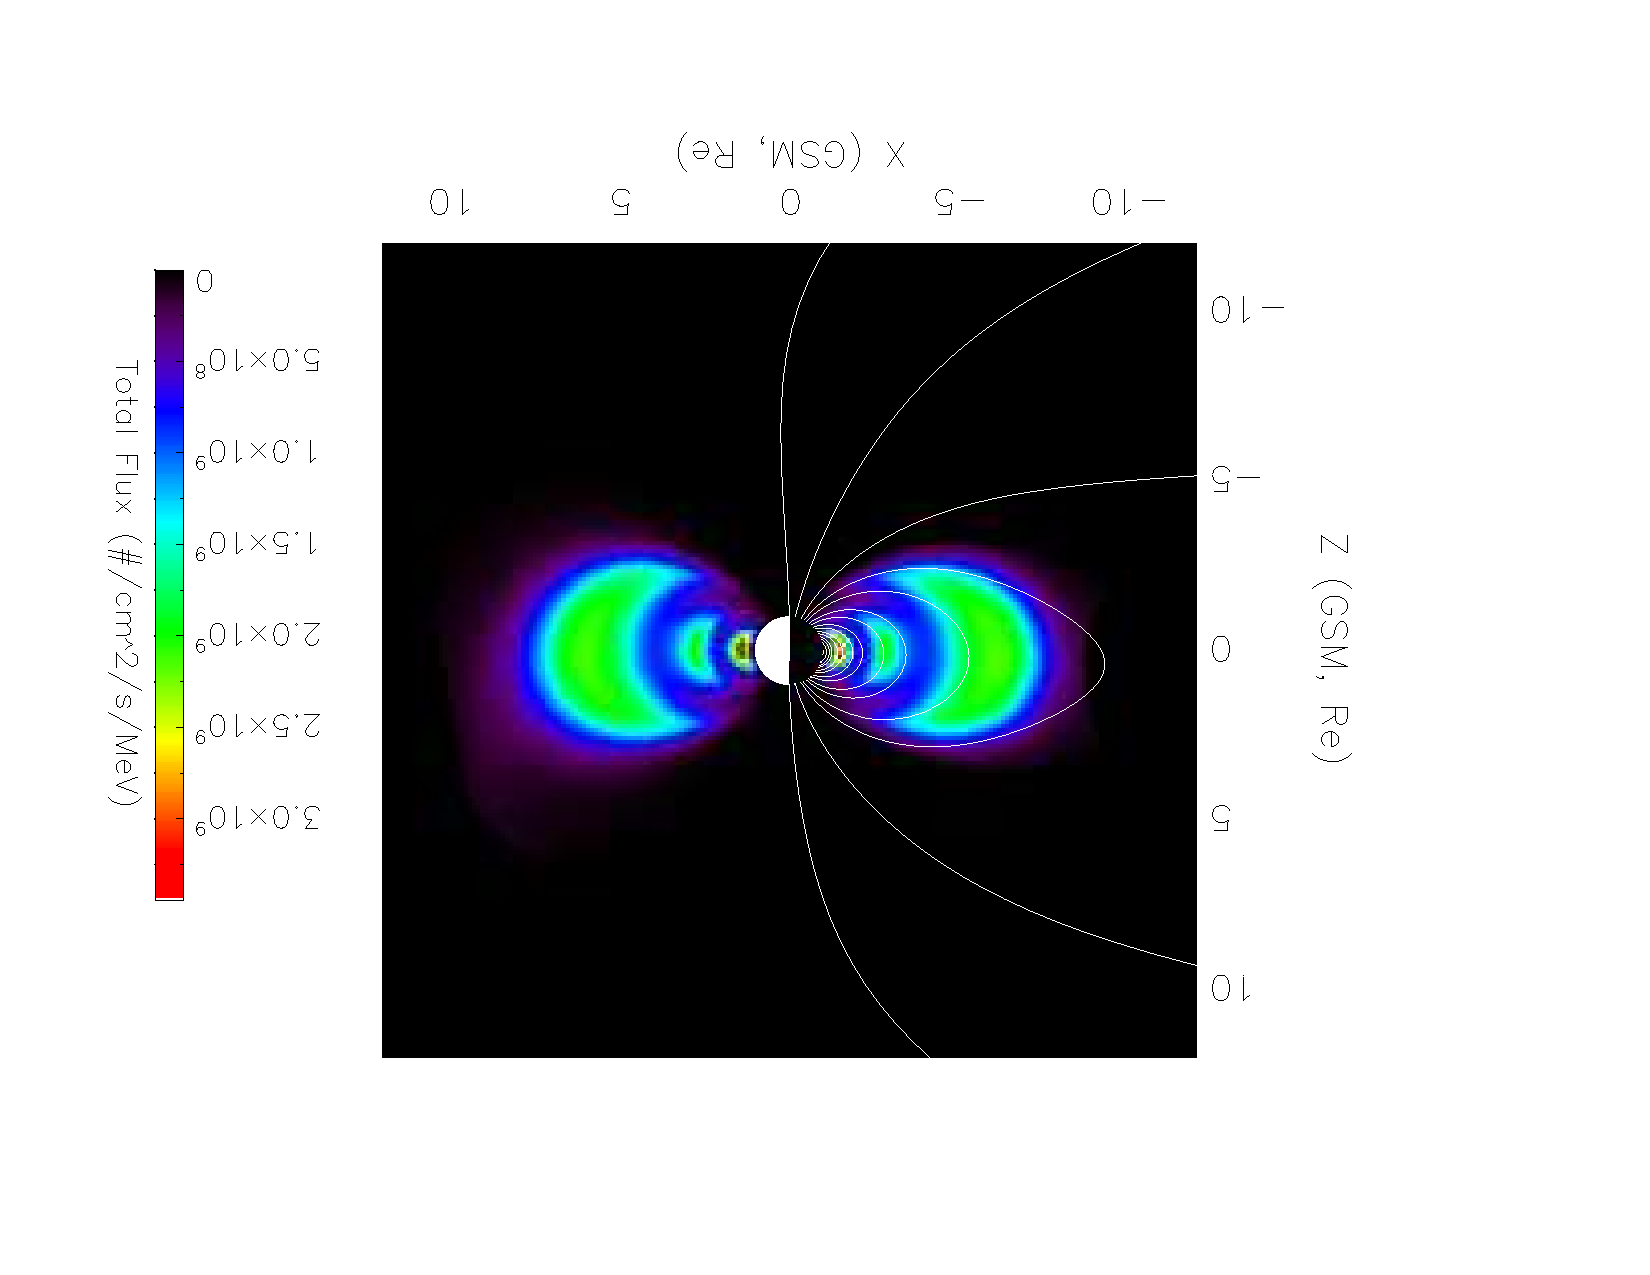
\includegraphics[width=1.0\textwidth,angle=180]{figures/chapter_2/radbelts_structure/radmodel}
\caption{Cutaway view of AE9 model electron fluxes in the radiation belts, with some model magnetic field lines from ~\cite{tsyganenko97} to show the overall geometry.}
\end{figure}

The main process which is thought to be responsible, at least partially, for the existsnce of the inner radiation belt is called cosmic ray albedo neutron decay (CRAND)~\citep{singer1958}. In the CRAND process, cosmic rays from space create neutrons in the upper atmosphere, which are then free to travel upwards, or downwards. Those which travel upwards, and subsequently decay into a proton and an electron, form the inner radiation belt. The gap that defines the separation of the inner and outer radiation belts is called the slot region, and is caused by a kind of radio wave called plasmaspheric hiss. As the radio wave interacts with particles trapped in the slot region it changes their motion in such a way that they precipitate and are lost in the Earth’s atmosphere. This process can be partially understood through the adiabatic description of trapped particle motion, which is discussed in the next section. Even though steady-state and adiabatic expressions of the process by which the slot region is formed make predictions that agree with experimental data, they do not form a complete description. 

 \section{Single Particle Motion}
 
 Some properties of the radiation belts, and electron precipitation, can be understood through a picture of their dynamics which considers particles independently. In this description, particle motions do not affect each other and we ignore the fact that a charged particle moving an an electromagnetic field also creates an electromagnetic field due to its own motion. This picture neglects the collective effects characteristic of space plasmas. 
 
Electrons from the radiation belts move under the influence of the Earths magnetic field. They are subject to the Lorentz force, $\mathbf{F} = q(\mathbf{E} + \mathbf{v}\times\mathbf{B})$, where $q$ is the electron charge, $\mathbf{v}$ is the velocity vector, and $\mathbf{B}$ is the static magnetic field. The Lorentz force causes cycloidal motion about lines of constant magnetic force. The velocity vector of the electrons can be expressed in components which are parallel and perpendicular to the local magnetic field. The parallel component of the velocity vector will be constant provided the fields $\mathbf{E}$ and $\mathbf{B}$ are constant. Only the electric field does work and changes the kinetic energy of the electrons. In this case the particle motion is a helix, with a pitch angle defined by:

$$\alpha = tan^{-1}\left(\frac{v_\perp}{v_\parallel}\right).$$

Particle motion in geospace can be described by adiabatic invariants, which are quantities that remain constant under slow changes to the system relative to the periodic motion of the particles. The action integral:

$$J = \oint p dq$$

is a constant of motion under these circumstances, where $p$ and $q$ are the generalized momentum and coordinate from Hamiltonian mechanics. It can be shown that the magnetic moment of an electron undergoing gyro motion is an adiabatic invariant. It follows that the magnetic flux encircled by the gyrating electron is also invariant. This quantity:

$$\Phi = \frac{2\pi m}{q^2}\mu$$

is called the first adiabatic invariant, where $q$ is the electron charge, $m$ is the electron mass, and $\mu$ is the magnetic flux enclosed by the electron gyro radius. The invariance of $\Phi$ implies that when an electron moves to a region of increased magnetic field strength, the gyro radius will decrease to encircle  a constant magnetic flux. For electrons in near Earth space, this means that the electron gyro radius decreases with proximity to the poles. This has the effect of creating a magnetic mirror, since the only parameter that can change in the magnetic moment:

$$\mu = \frac{mv^2 \sin^2(\alpha)}{2B}$$

is the pitch angle $\alpha$ given that kinetic energy is constant. The pitch angle $\alpha$ changes between values $\alpha_1$, $\alpha_2$ for magnetic field strengths $B_1$, $B_2$ according to:

$$\frac{\sin^2{\alpha_1}}{\sin^2{\alpha_2}} = \frac{B_2}{B_1}.$$

When an electron drifts towards a region of higher magnetic field strength, there will be a point where the pitch angle reaches $90^\circ$ and the parallel component of the velocity is zero. The force caused by the gradient in the magnetic field then accelerates the electron in the reverse direction. The point where this happens is called the mirror point. In the absence of other forces, electrons in near-Earth space undergo bounce motion between conjugate mirror points at the poles. When the mirror point occurs at a height inside the atmosphere, the electron will be absorbed and lost. The minimum magnetic field strength for an electron undergoing bounce motion occurs at the magnetic equator. Electrons with a pitch angle of nearly $90^\circ$ at the equator cannot move farther towards the poles, while electrons with pitch angles near $0^\circ$ can move unimpeded by the mirror force. The set of pitch angles at the equator which result in mirror points within the atmosphere are called the loss cone. Electrons with equatorial pitch angles within the loss cone will not undergo subsequent bounce motion and will precipitate into the atmosphere due to collisions with its neutral constituents.

\section{Scattering Processes}

Interactions with electromagnetic waves can change the pitch angles of electrons so that they lie within the loss cone and subsequently precipitate. When a wave phenomenon has a doppler-shifted frequency $\omega$ which is resonant with the relativistic electron gyro frequency, energy can be exchanged in a resonant interaction. This condition is written as:

$$\omega - k_{\parallel}v_{\parallel} = \frac{n\Omega_e}{\gamma}$$

where $k_{\parallel}$ and $v_{\parallel}$ are the parallel components of the wave vector and velocity vector, n is an integer multiple, $\gamma$ is the relativistic factor, and $\Omega_e$ is the electron cyclotron frequency. The resonant condition depends on the electron kinetic energy, and so different electromagnetic waves will resonantly interact with electrons that have a compatible energy range. This fact connects wave particle interactions in space to the population of electrons which precipitate into the atmosphere. Information about the scattering processes is carried by the precipitating electrons to the atmosphere. There are three main types of wave which are responsible for causing pitch angle scattering and electron precipitation. The first two we will discuss, plasmaspheric hiss, and whistler chorus, are different manifestations of the same type of wave propagation, called whistler-mode. 

Whistler-mode waves are right-hand circularly polarized waves which occur below the electron cyclotron frequency, $f_{\mbox{ce}}$. The dispersion relation for whistler mode propagation determines how the frequency $\omega$, is related to the wavenumber $k$, of the whistler mode waves. The derivation is accomplished using the theory of radio propagation through cold plasmas and several approximations, and results in the relation:

$$\frac{c^2k^2}{\omega^2} = 1 - \frac{{\omega_{pe}}^2}{\omega(\omega - |\Omega_e|)}$$

where $c$ is the speed of light, $k$ and $\omega$ are the is the wave number and frequency of the radio wave, $\omega_{pe}$ is the electron plasma frequency, and $\Omega_e$ is the electron gyro frequency. The plasma frequency $\omega_{pe}$ is given by:

$$\omega_{pe} = \sqrt{N e^2/\epsilon_0 m}$$

where $N$ is the electron number density, $e$ is the electron charge, and $m$ is the electron mass. The plasma frequency can be thought of as a natural frequency which the positive and negatively charged components of the plasma would oscillate at if there were separated by some small distance and released. A spectrogram showing how a typical whistler wave changes frequency in time is contained in Figure~\ref{whistler_spectrogram}, reproduced from data by the Stanford University VLF group. The radio receiver used to record these data were located at Palmer Station, Antarctica.

\begin{figure}[p]
\label{whistler_spectrogram}
\centering
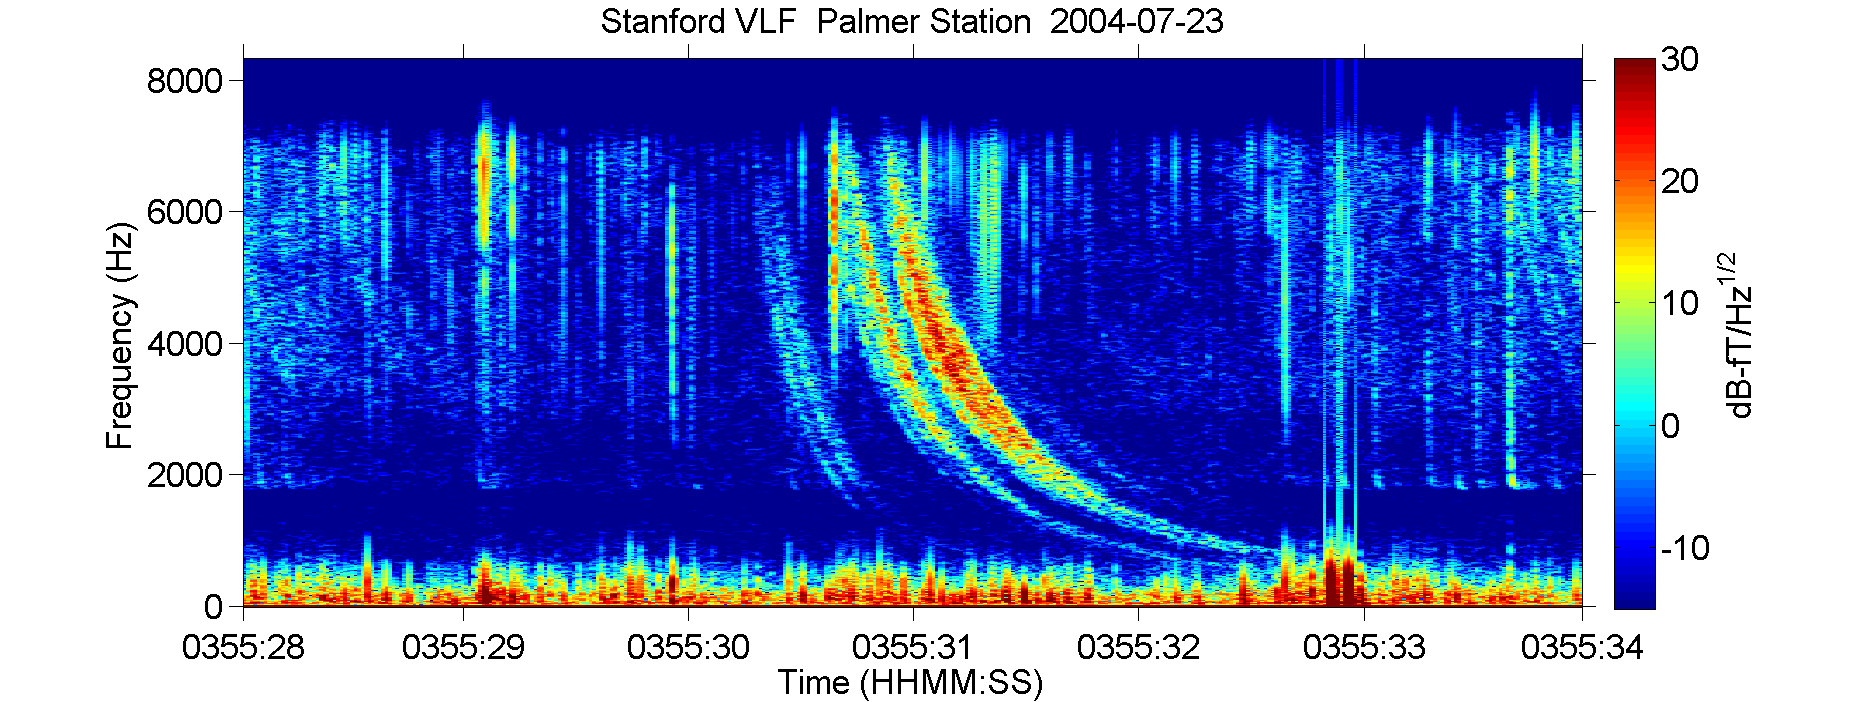
\includegraphics[width=1.0\textwidth,angle=0]{figures/chapter_2/whistler/Whistler_radio_palmer_2004-07-23_T035528.png}
\caption{Frequency/time relation for a whistler-mode wave, observed by a Stanford University VLF radio receiver at Palmer Station, Antarctica.}
\end{figure}


A key driver of electron precipitation is plasmaspheric hiss, which is a particular kind of whistler-mode wave that is responsible for the formation of the slot region in the radiation belts~\citep{lyons1972, lyons1973}. The frequency range is broadband ELF, occupying 100 Hz to a few KHz~\citep{millan2007}. The generation mechanism is not fully understood. Theoretical modelling is consistent with generation by the electron cyclotron instability~\citep{millan2007, huang1983, church1983, meredith04}. The electron cyclotron instability, described by~\cite{thorne1979a}, was known in plasma physics before plasmaspheric hiss was discovered~\citep{kennel1966}, and is a way that the local plasma population can create hiss. At the time of writing, it is thought that there are several distinct mechanisms which combine to produce plasmaspheric hiss in different situations~\citep{thorne2010,bortnick2008,bortnick2009}.. Hiss below frequencies of 150 Hz is thought to be generated by amplification of whistler-mode noise due to substorm-injected electrons~\citep{meridith2018}. At higher frequencies, up to approximately 2 Khz, hiss likely comes from short bursts of chorus emissions (discussed next), which exist farther out in space, propagate in, and become trapped in the plasmasphere~\citep{meridith2018}. Finally, at higher frequencies, hiss becomes more associated with land mass and geographic location, which suggests an association with terrestrial lightning. 

Another important wave phenomenon which causes precipitation is whistler mode chorus. Chorus is a wave phenomenon consisting of discrete whistler-mode emissions, which are observed outside the plasmasphere, with a frequency range of 100 Hz to 5 Khz~\citep{millan2007}. The waves occur in two distinct bands, one below, and one above, half the electron gyro frequency~\citep{Tsurutani1974,thorne2010}. It is believed that chorus is generated by the electron-cyclotron instability from injected plasma sheet electrons near the equator~\citep{kennel1966,millan2007}. Chorus waves cause a phenomenon called microburst precipitation~\citep{millan2007}. Microburst precipitation is characterized by short, quasi-periodic bursts of electron precipitation that occur on timescales of 10 milliseconds. Microbursts were first discovered at relatively low energies (approximately 100 KeV), but they do occur at relativistic, MeV energies as well. The relation between microburst precipitation and chorus waves is suggested by the fact that they both occur between 0300 and 1500 magnetic local time~\citep{lorentzen2001,millan2007}, and spacecraft measurements of both phenomena showed a strong correlation. An investigation by~\citet{thorne2005} used data from a 1998 geomagnetic storm event to estimate the microburst precipitation rate due to whistler mode chorus waves and found general agreement between between observed, and model, loss rates at wave amplitudes consistent with observations~\citet{millan2007}.

Chorus waves are an important loss mechanism for the radiation belts. Pitch angle scattering caused by chorus waves occurs over a broad range of energies~\citet{thorne2010}, from tens of keV to MeV. There are limits to the applicability of the quasi-linear description of wave-particle interactions between electrons and chorus waves, which are relevant, because very large amplitude chorus waves have been observed, with electric field strengths of more than 240mV/m~\citep{cattell2008,thorne2010}. These cases, in particular, highlight the need for experimental measurements as constraints for implemented models. 

A different electromagnetic wave that causes precipitation is the Electron Ion Cyclotron (EMIC) Wave. EMIC waves are a distinct type of electromagnetic wave, which are left-hand circularly polarized with frequencies below the proton gyro frequency. EMIC waves occur in bands separated by multiples of the ion gyrofrequency~\citep{thorne2010}. Different ion species give rise to different frequencies for EMIC waves. These waves are thought to originate near the equator~\citep{fraser1996,lotouaniu2005,millan2007}, where they are created by a temperature anisotropy in the ring current with respect to the local magnetic field~\citep{jordanova2001}. EMIC waves are known to be a major source of loss for electrons in the radiation belts. At energies of greater than approximately several 100 keV, they are effective at scattering electrons into the loss cone~\citet{thorne1981,millan2007}.The resonance condition requires that the wave, which is left-hand circularly polarized, be seen in the electron frame as right-hand polarized. This happens when the electron overtakes the wave, and so requires the electrons to have a  minimum energy~\citet{millan2007}. This minimum energy required can be calculated from the dispersion relation of the EMIC wave.

Satellite observations suggest that, most of the time, precipitation caused by EMIC waves occurs at higher energies~\citep{millan2007}. This can be seen as a result of the fact that owing to their left-handed polarization, an electron scattered by an EMIC wave needs to have a kinetic energy high enough that it overtakes the wave and sees it as right-handed polarized in its reference frame. The survey conducted by~\citep{merideth2003} using measurements of EMIC waves by the CERES satellite found that the resonant energy required for electron scattering was less than 2 MeV in only approximately 11 percent of cases. The first balloon with a detector capable of measuring these higher energies was flown from 1996 in Kiruna, Sweden~\citep{millan2007}. This balloon measured electron precipitation with a peak characteristic energy of 1.7 MeV~\citep{foat1998}. The observed precipitation was later shown by~\citep{lorentzen2000} to be associated with nearby spacecraft observations of EMIC waves~\citet{millan2007}.

The different types of wave that result in electron scattering and precipitation are energy selective, applying to populations of electrons with distinct energy ranges. This implies that information about the scattering processes can be found by measuring the properties of electrons which precipitate to the atmosphere. The focus of this thesis is on experimental techniques that can be used to accomplish this.

